% !TeX encoding = UTF-8
% !TeX root = ../main.tex

\section{CPS到SSA转换过程的验证}

\begin{frame}{基于模拟技术的验证}
    我们需要使用模拟技术证明:\\
    \vspace{1ex}
    目标程序\textcolor{DarkBlue}{保存}了源程序的\textcolor{DarkBlue}{语义},即目标程序的行为是可接受的源程序行为。
    \begin{figure}
        \centering
        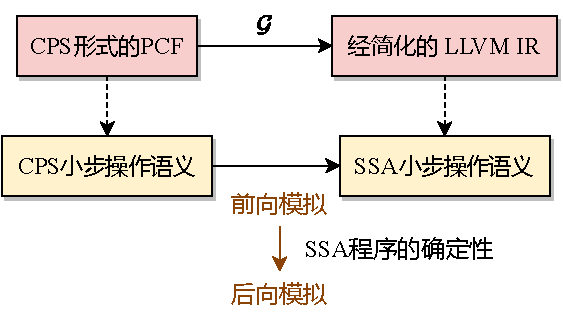
\includegraphics[width=0.55\linewidth]{figures/extracts.pdf}
    \end{figure}
\end{frame}

\begin{frame}{小步操作语义}
    \large
    \textcolor{DarkBlue}{CPS小步操作语义}\\
    \normalsize
    \vspace{1ex}
    \centering
    CPS程序状态之间的一步转换:$(t_{cps},loc_{cps})\rightarrow(t'_{cps},loc'_{cps})$\\
    \vspace{1ex}
    转换规则:
    $\displaystyle{\frac{loc_{cps}\; k = (\mathbf{letcont}\; k\; x=t_1\; \mathbf{in}\; t_2)}{(k\; v,\; loc_{cps})\rightarrow (t_1 [v/x],\; loc_{cps})}}$ \\
    \vspace{1ex}
    ...\\
    % \vspace{1ex}
    \flushleft
    \textcolor{DarkBlue}{SSA小步操作语义}\\
    \vspace{1ex}
    \centering
    SSA程序状态之间的一步转换:$(pc,ppc,loc_{ssa},s_{ssa})\rightarrow (pc',ppc',loc'_{ssa},s'_{ssa})$\\
    \vspace{1ex}
    % \flushleft 
    % 转换规则:\\
    \centering 
    转换规则:
    $\displaystyle{\frac{\mathbf{code}_{at}\; pc\; =\; (y=\mathbf{call}\; f\; v_0)\quad \mathbf{arg}\; f = x}{(pc,\; ppc,\; loc_{ssa},\; s_{ssa})\rightarrow ((f,b_1,0),\; pc,\; loc_{ssa}\; [x\mapsto v_0],\; \mathbf{push}\; s_{ssa}\; pc )}}$ \\
    \vspace{1ex}
     ...\\
\end{frame}

\begin{frame}{CPS到SSA的前向模拟}
    \begin{figure}
        \centering
        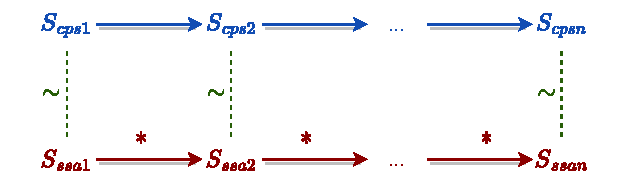
\includegraphics[width=0.65\linewidth]{figures/star.drawio.pdf}
    \end{figure}
    \begin{enumerate}
    \item \textcolor{DarkBlue}{CPS}和\textcolor{Maroon}{SSA}程序状态之间的不变式: \textcolor{DarkBlue}{$S_{cps}\sim S_{ssa}$}
    \item 初始状态:\textcolor{DarkBlue}{$\mathtt{initial}\; (t_{cps}) \sim \mathtt{initial}\; (t_{ssa})$}
    \item 程序内部执行步骤的模拟:星形模拟。对CPS程序状态的一步转换进行归纳。
    \item 不变式在程序执行结束时仍成立。
\end{enumerate}
\end{frame}

\begin{frame}{防止无限驻留}  
    \begin{figure}
        \centering
        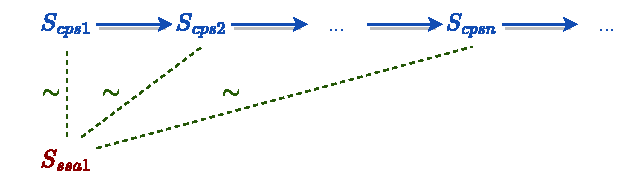
\includegraphics[width=0.65\linewidth]{figures/stutter.drawio.pdf}
    \end{figure}
    \begin{itemize}
        \item 处理$\mathbf{letcont}$代码项时SSA程序状态会驻留。
        \item 为了防止无限驻留,需要为CPS程序状态定义度量函数$M$。
        \item $M$严格递减:$S_{cps1}\rightarrow S_{cps2},\  M(S_{cps1})>M(S_{cps2})$.
        \item 使用$\mathbf{letcont}$代码项的数量作为$M$.
    \end{itemize}
\end{frame}

\begin{frame}{CPS到SSA的前向模拟示例}
    \small
\begin{columns}[t, onlytextwidth]
    \column{0.4\textwidth}
    \textcolor{DarkBlue}{CPS程序}\\
    $\quad  (\mathbf{letcont}\; k_2\; y= k_{init}\; y\; \mathbf{in}$\\
    $\quad\quad  \textcolor{Maroon}{(f\; k_2\; x_3)})$\\
    \column{0.6\textwidth}
    \textcolor{DarkBlue}{SSA程序}\\
    $\mathbf{define}\; main\; ( )$\\
    $\quad b_1:\; x_3 = 2;\;$
    \textcolor{Maroon}{$ y = \mathbf{call}\; f\; x_3;\; \mathbf{br_{uc}}\; k_2;$}\\
    $\quad k_2:\; r_{k2} = y;\; \mathbf{ret}\; r_{k2};$ \\
\end{columns}
    \small
    $\textcolor{DarkBlue}{S_{cps1}}:\; ((f\; k_2\; x_3),\, loc)$\\
    $\textcolor{Maroon}{S_{ssa1}}:\; (t_{ssa},\, (main, b_1, 1),\, (main, empty, 0),\, loc_{ssa},\, s_{empty})$\\
    \vspace{1ex}
    \invisible{$\textcolor{DarkBlue}{S_{cps2}}:\; ((k_{init}\; y),\, loc\; [k_2\mapsto t_{cps}])$\\
    $\textcolor{Maroon}{S_{ssa2}}:\; (t_{ssa},\, (main, k_2, 0),\, (main, b_1, 1),\, loc_{ssa},\, s_{empty})$}\\
    \begin{figure}
        \centering
        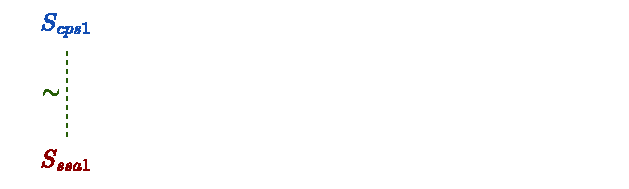
\includegraphics[width=0.6\linewidth]{figures/star1.drawio.pdf}
    \end{figure}
\end{frame}

\begin{frame}{CPS到SSA的前向模拟示例}
    \small
\begin{columns}[t, onlytextwidth]
    \column{0.4\textwidth}
    \textcolor{DarkBlue}{CPS程序}\\
    $\quad  (\mathbf{letcont}\; k_2\; y= \textcolor{Maroon}{k_{init}\; y}\; \mathbf{in}$\\
    $\quad\quad  \textcolor{Maroon}{(f\; k_2\; x_3)})$\\
    \column{0.6\textwidth}
    \textcolor{DarkBlue}{SSA程序}\\
    $\mathbf{define}\; main\; ( )$\\
    $\quad b_1:\; x_3 = 2;\;$
    \textcolor{Maroon}{$ y = \mathbf{call}\; f\; x_3;\; \mathbf{br_{uc}}\; k_2;$}\\
    $\quad k_2:\; \textcolor{Maroon}{r_{k2} = y;\; \mathbf{ret}\; r_{k2};}$ \\
\end{columns}
    $\textcolor{DarkBlue}{S_{cps1}}:\; ((f\; k_2\; x_3),\, loc)$\\
    $\textcolor{Maroon}{S_{ssa1}}:\; (t_{ssa},\, (main, b_1, 1),\, (main, empty, 0),\, loc_{ssa},\, s_{empty})$\\
    \vspace{1ex}
    $\textcolor{DarkBlue}{S_{cps2}}:\; ((k_{init}\; y),\, loc\; [k_2\mapsto t_{cps}])$\\
    $\textcolor{Maroon}{S_{ssa2}}:\; (t_{ssa},\, (main, k_2, 0),\, (main, b_1, 1),\, loc_{ssa},\, s_{empty})$\\
    \begin{figure}
        \centering
        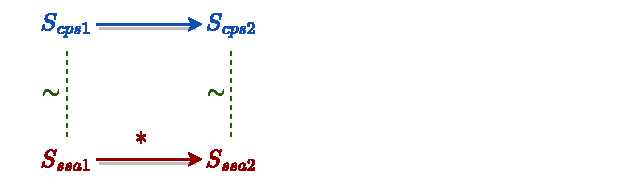
\includegraphics[width=0.6\linewidth]{figures/star2.drawio.pdf}
    \end{figure}
\end{frame}

\begin{frame}{CPS到SSA的前向模拟示例}
    \small
\begin{columns}[t, onlytextwidth]
    \column{0.4\textwidth}
    \textcolor{DarkBlue}{CPS程序}\\
    \textcolor{Maroon}{$\quad  (\mathbf{letcont}\; k_2\; y= k_{init}\; y\; \mathbf{in}$\\
    $\quad\quad  (f\; k_2\; x_3))$}\\
    \column{0.6\textwidth}
    \textcolor{DarkBlue}{SSA程序}\\
    $\mathbf{define}\; main\; ( )$\\
    $\quad b_1:\; x_3 = 2;\;$
    \textcolor{Maroon}{$ y = \mathbf{call}\; f\; x_3;\; \mathbf{br_{uc}}\; k_2;$\\
    $\quad k_2:\; r_{k2} = y;\; \mathbf{ret}\; r_{k2};$} \\
\end{columns}
    $\textcolor{DarkBlue}{S_{cps1}}:\; ((f\; k_2\; x_3),\, loc)$\\
    $\textcolor{Maroon}{S_{ssa1}}:\; (t_{ssa},\, (main, b_1, 1),\, (main, empty, 0),\, loc_{ssa},\, s_{empty})$\\
    \vspace{1ex}
    $\textcolor{DarkBlue}{S_{cps2}}:\; ((k_{init}\; y),\, loc\; [k_2\mapsto t_{cps}])$\\
    $\textcolor{Maroon}{S_{ssa2}}:\; (t_{ssa},\, (main, k_2, 0),\, (main, b_1, 1),\, loc_{ssa},\, s_{empty})$\\
    \begin{figure}
        \centering
        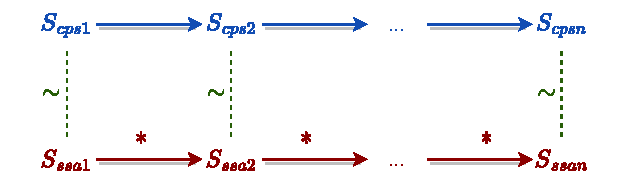
\includegraphics[width=0.6\linewidth]{figures/star.drawio.pdf}
    \end{figure}
\end{frame}

